As a final look at the HEG, we can attempt to calculate the correlation energy per electron in the thermodynamic limit using the formalism developed in the previous chapter. We have used 14 training points, from N = 2 to N = 502, and an SRE sequence length of 3. Again, the machine learning algorithm used to make these predictions is the Bayesian Ridge regression algorithm. We attempted this extrapolation using the correlation energies, which have been fully calculated at M = 6,142, and the correlation energies, which have been predicted by the SRE method and are shown in Fig. \ref{brr_eg}.  However, these two extrapolations result in identical correlation energies, with a percent error between the two extrapolated data sets being 0.0$\%$. Thus, there is no reason to use the fully calculated data to predict the TDL correlation energies when the SRE predictions result in the same answer and yield significant time savings.

Fig. \ref{fig:TDL_all} shows the correlation energies per particle for the HEG at a variety of values for N and $r_s$ with solid lines. The horizontal dashed lines show the correlation energy at the TDL as predicted by the SRE algorithm. Even though the correlation energies show significant oscillations with respect to the number of electrons in the system (likely due to the periodic boundary conditions), the SRE predictions seem to provide a suitable match for where the oscillations will converge.

\begin{figure}
    \centering
    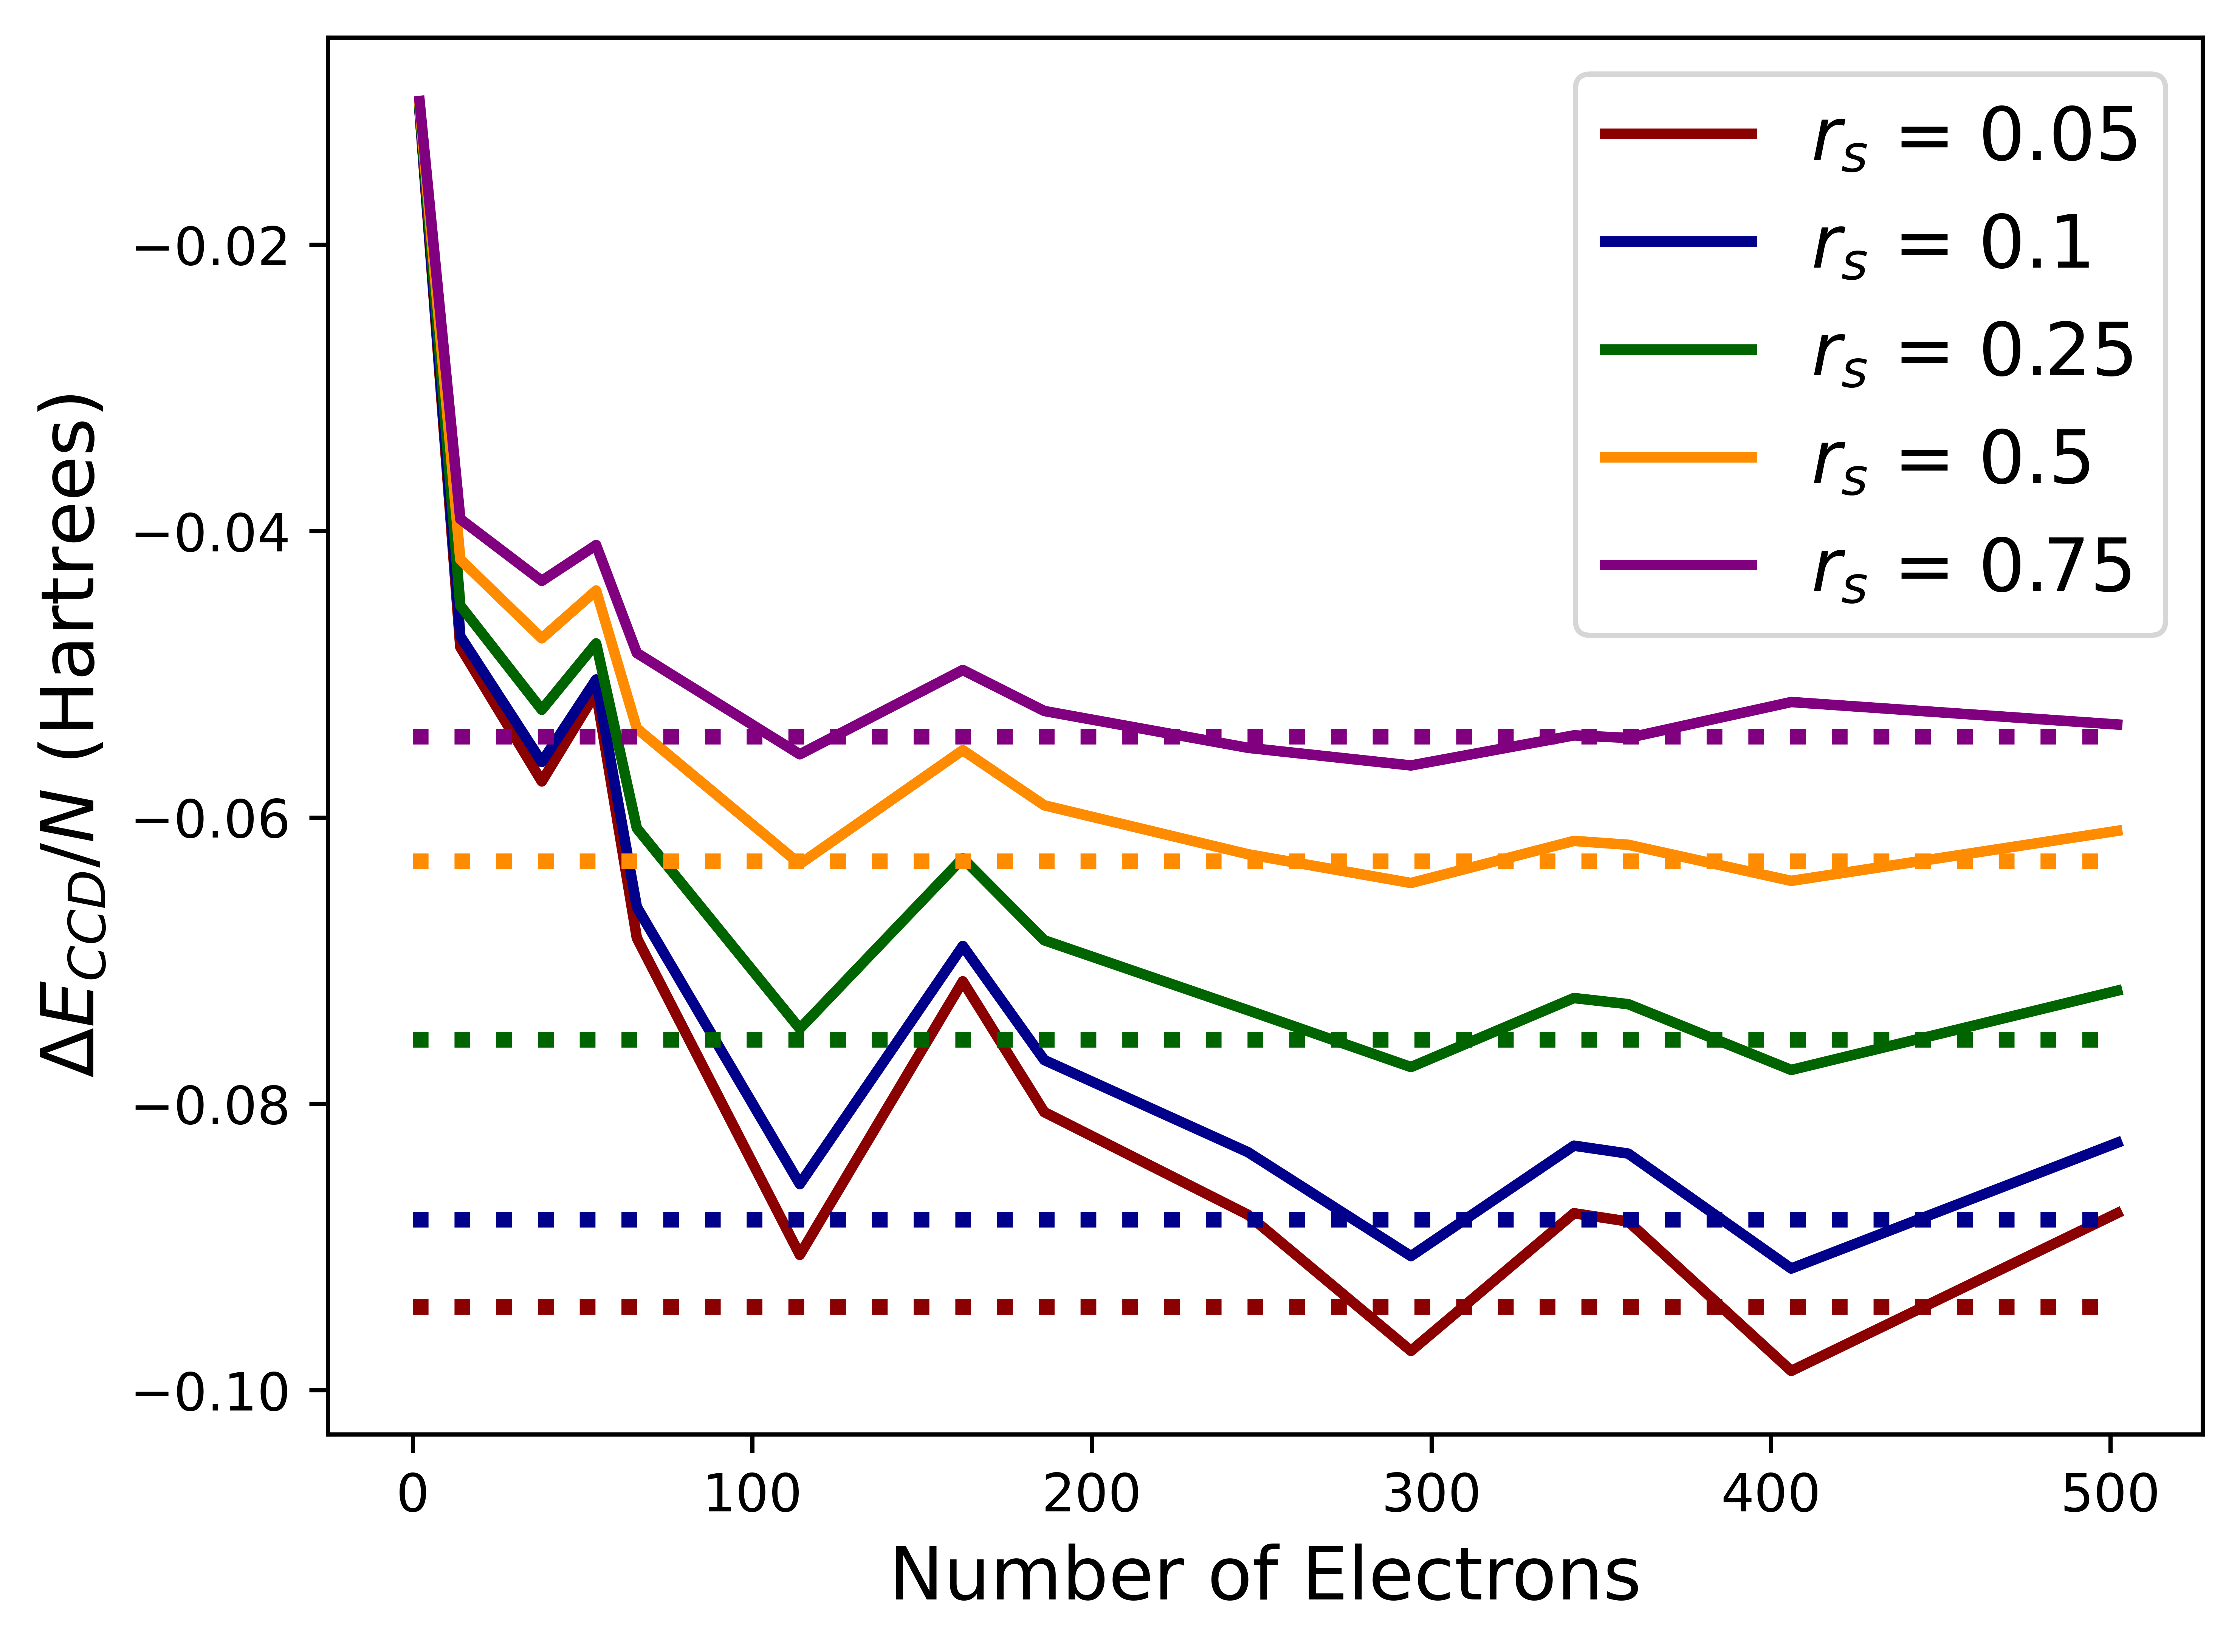
\includegraphics[scale=0.75]{Images/Chapter7/ElectronGas/TDL_all.png}
    \caption{The converged CCD correlation energies for the HEG calculated at M = 6,142 (solid) and the TDL predictions for the correlation energy per particle calculated through the SRE method (dashed).}
    \label{fig:TDL_all}
\end{figure}

While there do exist literature values for the HEG in the TDL (for example, see the work by Bishop et al. in \cite{Ref71} and \cite{Ref72}), the results are highly dependent on the many-body method used, the values of $r_s$ studies, and the specifications of the HEG system. Thus we could not find any currently published literature results to compare our predictions for the exact specifications we have reported. However, we can use a power law, a standard method to find the TDL energies (see Ref. REFERENCE HERE). Therefore, we will use a power law of the form:

\begin{equation}
    \Delta E_{CCD}(N) = \Delta E_{CCD}^\infty + AN^{-\alpha},
\end{equation}

where $\Delta E_{CCD}^\infty$, A, and $\alpha$ are parameters that are fit using data generated at finite numbers of electrons and $\Delta E_{CCD}^\infty$ the is correlation energy at the thermodynamic limit. Usually, $\alpha$ is fixed to 1, which is used when calculating the correlation energy for the system at the TDL. We, however, are interested in calculating the correlation energy in the TDL per electron and thus will leave $\alpha$ unfixed. The results for performing this power law fit are shown in Fig. \ref{fig:TDL_0_5} for a HEG with $r_s$ = 0.5 and are also plotted with the SRE predictions for the correlation energy at the TDL from complete calculations and the SRE predictions. Also shown are the complete calculations for the finite numbers of electrons shown at M = 6,142. While it is impossible to say which of these results is the most accurate, it does appear that the SRE predictions visually provide a better matching for the convergence of the correlation energies in the TDL. However, the best method of predicting the correlation energies in the TDL and the error in the predictions is still a topic of ongoing research.


\begin{figure}
    \centering
    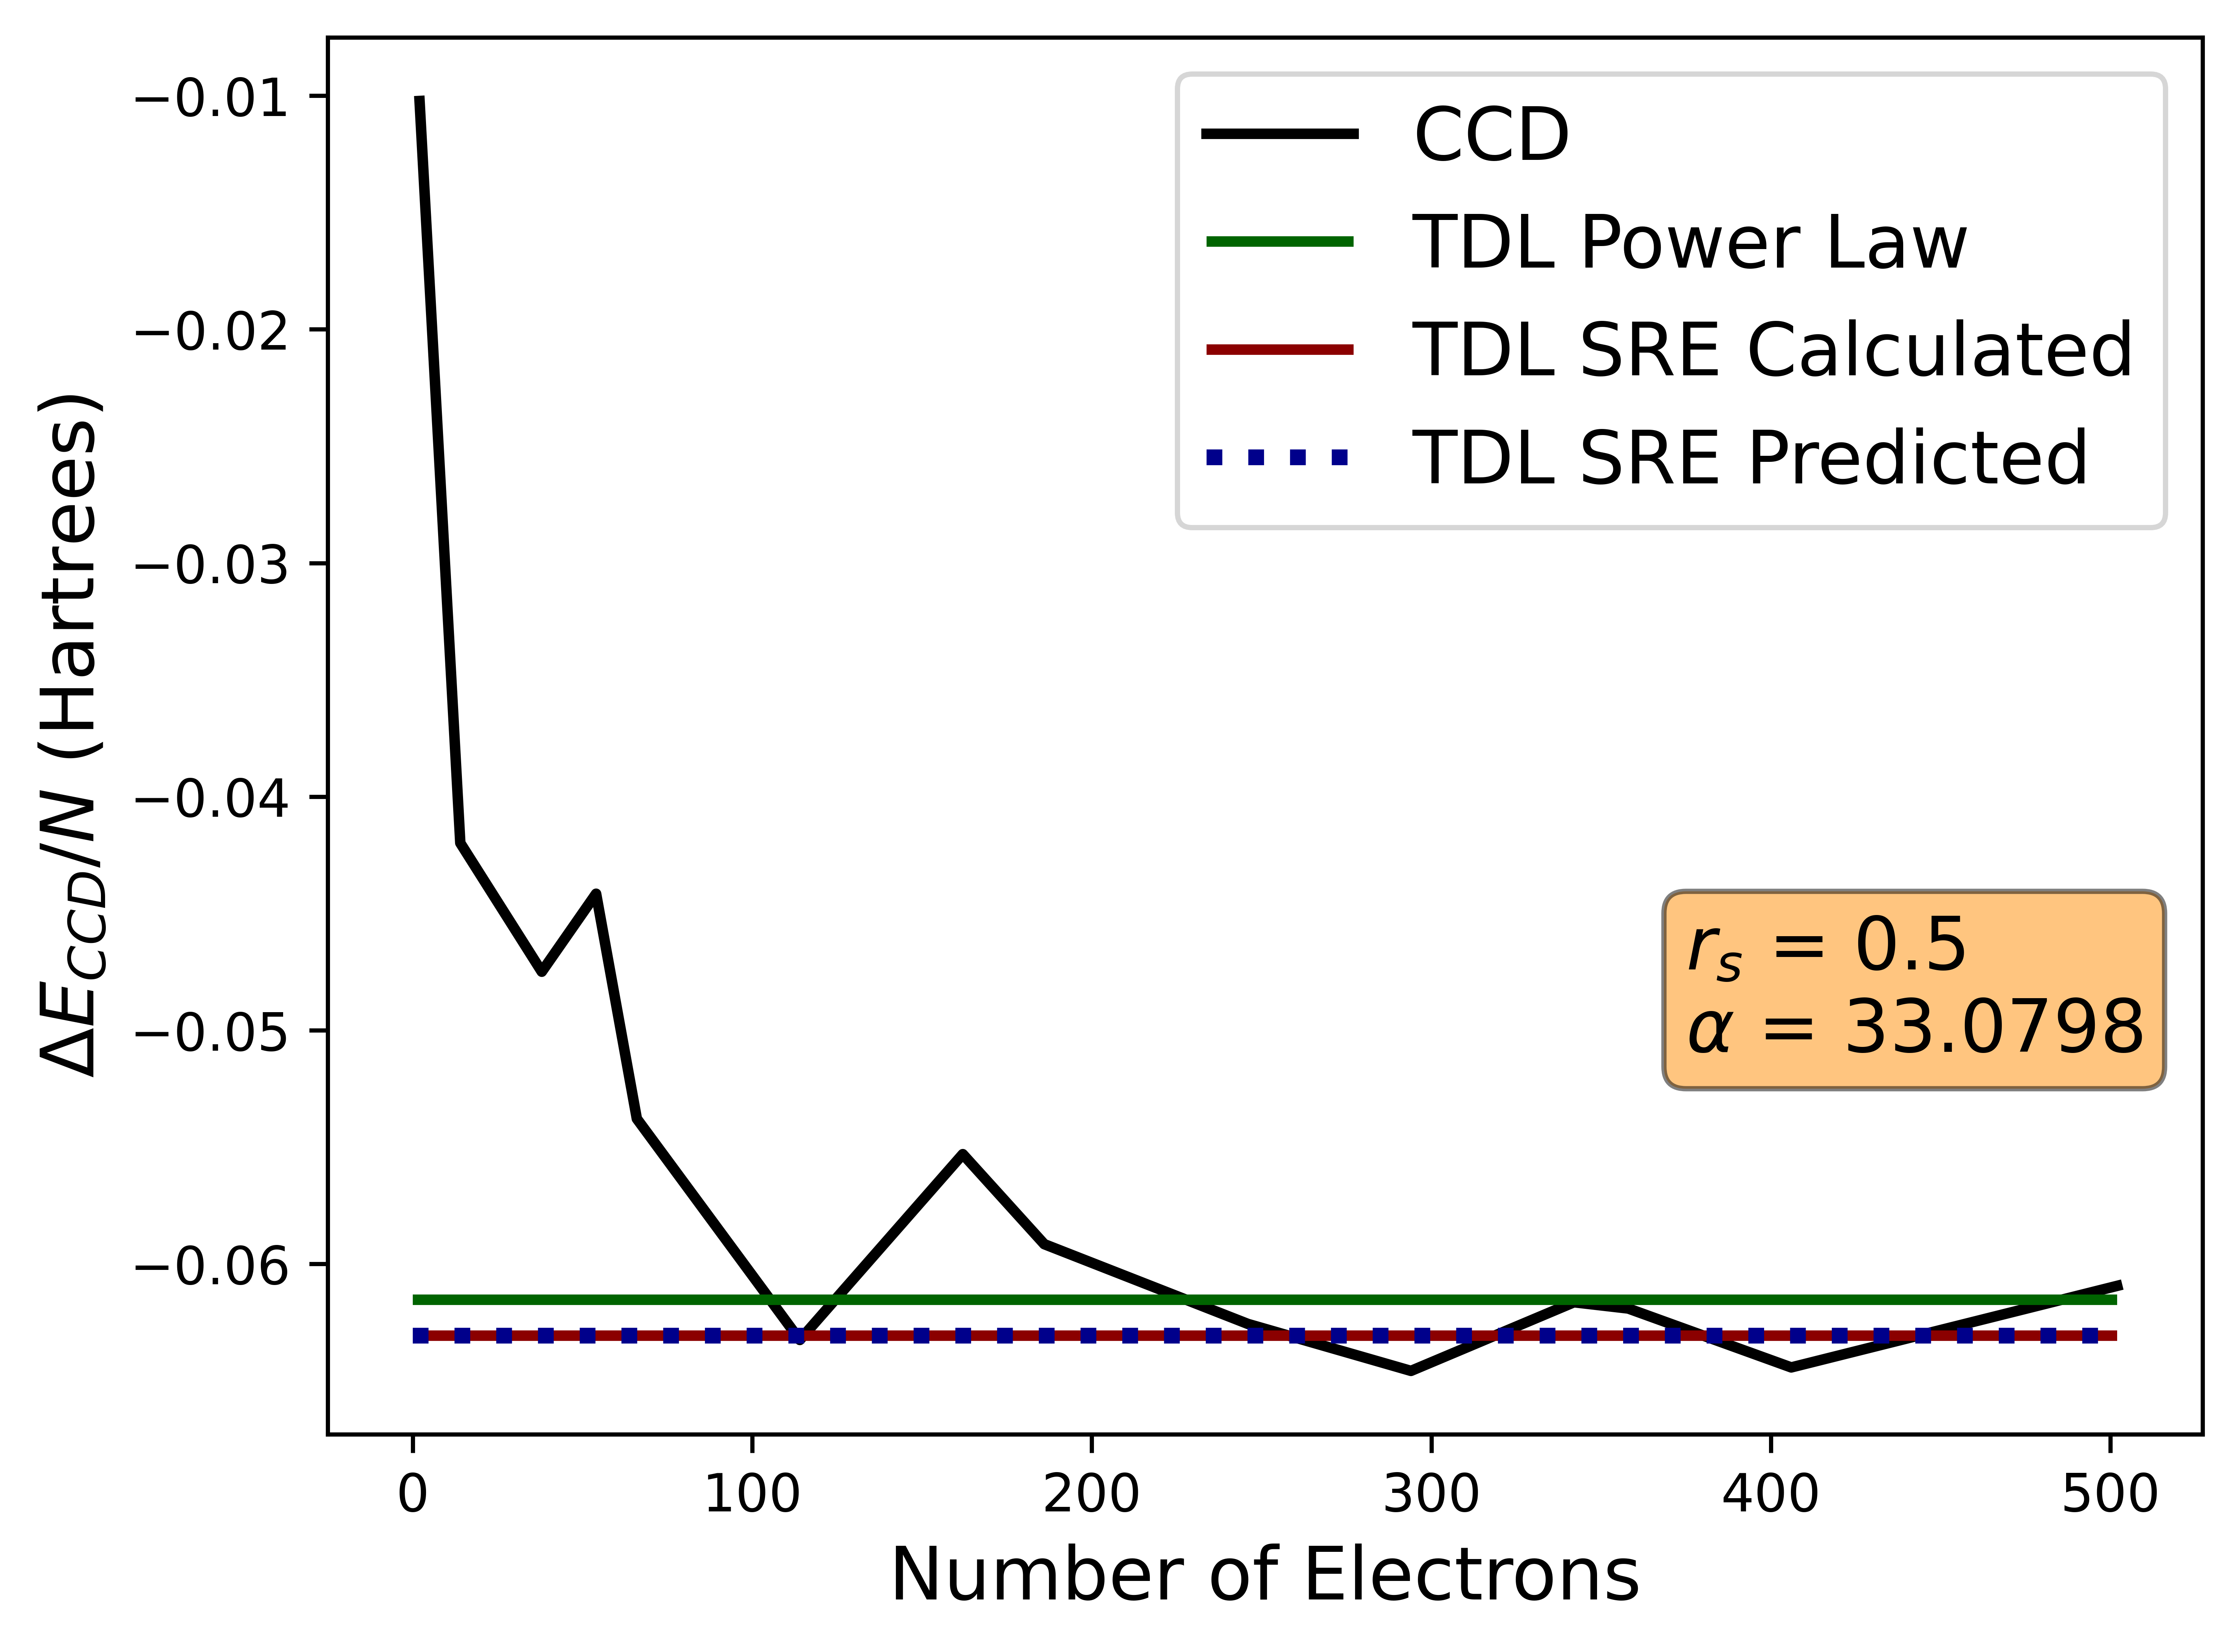
\includegraphics[scale=0.5]{Images/Chapter7/TDL_0.5.png}
    \caption{The CCD correlation energy per electron for an HEG with $r_s$ = 0.5 and calculated at M = 6,142 (black).  The power law prediction for the TDL correlation energy per electron is shown in green, and the SRE predictions for the TDL correlation energy per electron extrapolated from calculated and predicted energies are shown in red and blue, respectively.}
    \label{fig:TDL_0_5}
\end{figure}